\documentclass[fleqn,10pt]{./class/wlscirep}
\title{Analizing resource allocation for a distributed monitoring application}

\author[1,2,3,*]{Bogdan-Constantin Irimie}

\affil[1]{Institute e-Austria Timisoara, Romania}
\affil[2]{Department of Computer Science, West University of Timisoara, Romania}
\affil[3]{Department of Computing, Imperial College London, United Kingdon}
\affil[*]{bogdan.irimie90@e-uvt.ro}

\keywords{Resource allocation, performance monitoring}

\begin{abstract}
In a cloud environment monitoring applications should be able to scale in order to satisfy the monitoring requirements offering good quality of service and efficient resource utilization. In order for this scaling to be possible, monitoring applications should be built from the ground up with this goal in mind and mechanism for auto scaling should be implemented in order to provide a fast adaptation time. This report describes the work that has been done in order to enhance a monitoring system with automatic resource allocation capabilities. The work describes possible architectures with their advantages and drawbacks and implementations with their technical challenges.
\end{abstract}
\begin{document}

\flushbottom
\maketitle
\thispagestyle{empty}

\section*{Introduction}

Monitoring plays an important role in todays offerings of computing computing because it enables cloud providers and consumers to check if the quality of service they have agreed upon is satisfied, additionally monitoring can be used to verify that a certain level of security is enabled. 

Resources in the cloud can be provisioned and released with ease in a short period of time and monitoring systems should be able to scale just as fast in order to adapt to the new monitoring requirements. In order to adapt, the monitoring systems
should relay on a resource allocation mechanism that can take into account the architectures of the monitoring systems and provide strategies for resource allocation. The architecture of the monitoring systems is very important because it dictates the means of obtaining scalability, some systems having architectures that allow scaling with ease by providing decoupled systems where each component can be scaled independently,while other systems are build on a monolithic architecture making scaling more challenging and in some cases even impossible.

In this report we will focus on a monitoring system that implements a pipe and filter architecture allowing independent scaling of all components, and thus providing fault tolerance and parallel execution of jobs. 

\section{Analyzing the system and it's architecture}

The architecture Fig. \ref{fig:systemArchitecture} of the system is pr

\begin{figure}[ht]
\centering
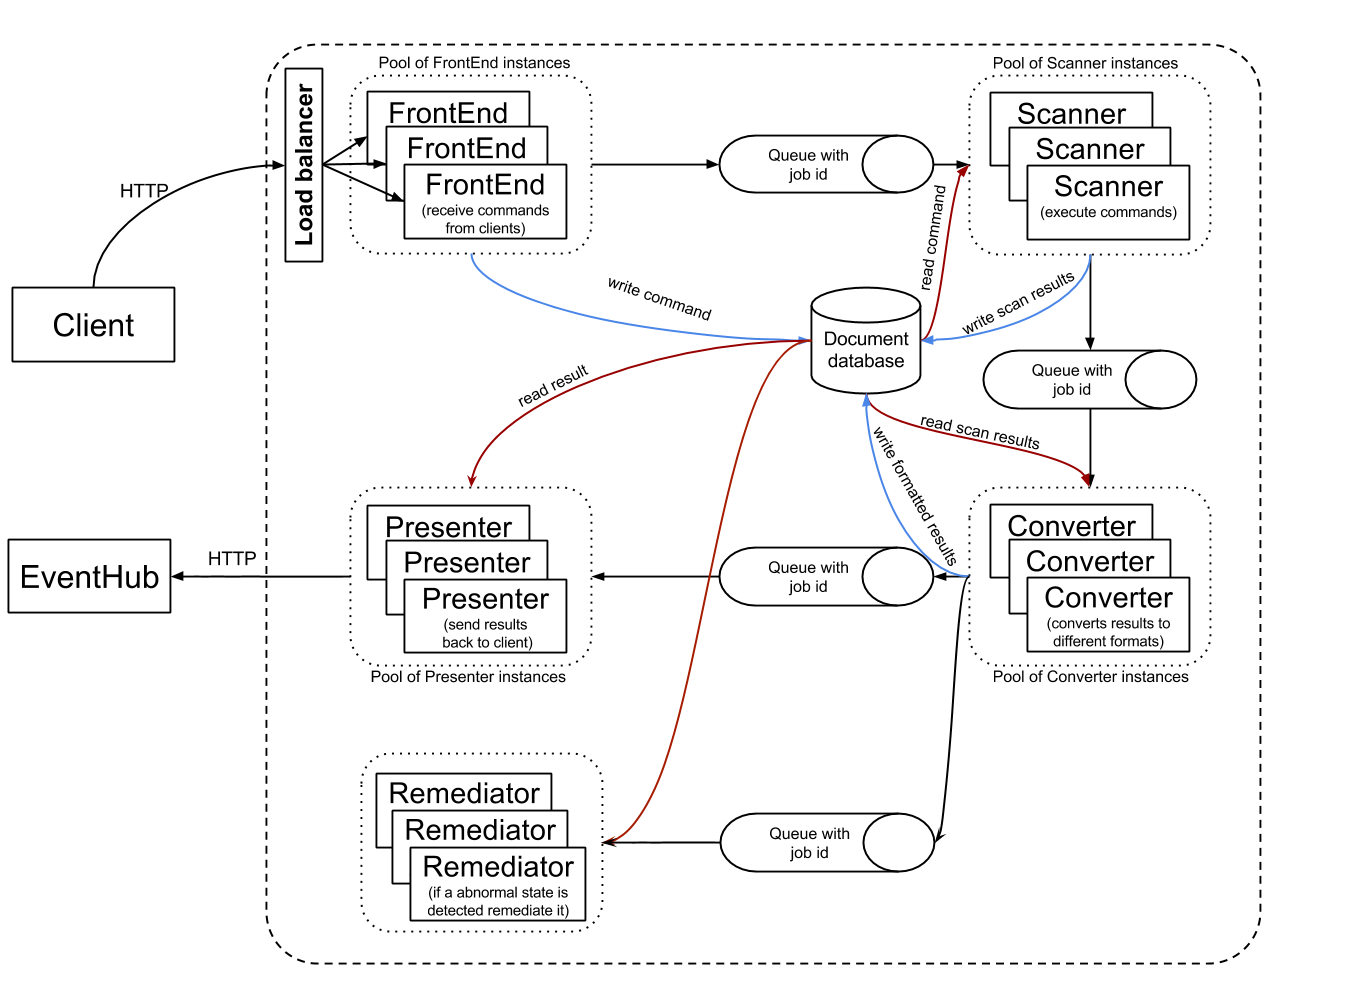
\includegraphics[width=\linewidth]{./img/MonitoringSystemArchitecture Remediation.png}
\caption{Distributed monitoring system architecture}
\label{fig:systemArchitecture}
\end{figure}



\bibliography{./bib/sample}

\section*{Acknowledgements}


\end{document}
